\documentclass[12pt]{article}
\usepackage{amsmath}
\usepackage{listings}
\usepackage{textcomp}
\usepackage{graphicx}
\graphicspath{ {../images/} }

\usepackage[utf8]{inputenc} % allow utf-8 input
\usepackage[T1]{fontenc}    % use 8-bit T1 fonts
\usepackage{hyperref}       % hyperlinks
\usepackage{url}            % simple URL typesetting
\usepackage{booktabs}       % professional-quality tables
\usepackage{amsfonts}       % blackboard math symbols
\usepackage{nicefrac}       % compact symbols for 1/2, etc.
\usepackage{microtype}      % microtypography
\setlength{\parindent}{0pt}

\title{Using ML Approach to NCAA Match Prediction}

\author{
\begin{tabular}{ccc}
Ming~Cheng & Xingwei~Ji & Xiaofang~Jiang  \\
Fangzhou~Li & Diwen~Lu & Paul~Lu \\
Jiayi~Xu & Timothy~Zhang & Haibin~Zhang \\
 & Feiwen~Zheng 
\end{tabular}
}

\begin{document}

\maketitle

\textbf{Github Link:}\\
https://github.com/3tz/Using-ML-Approach-to-NCAA-Match-Prediction

\begin{abstract}
\quad We are doing prediction on result of National Collegiate Athletic Association (NCAA) Basketball game. Data preprocessing was performed to generate pre-game (statistics of a Team or a player collected after a game) and post-game (expected statistics of a Team or a player before a game) statistics, while post-game statistics is used for feature validation. Then, we use logistic regression and MLP to predict the result for this year using data from previous years. The pre-game prediction use regular season matches since 2010 to predict the winner between any two teams in 2018. The post-game prediction relies on data from 2003 to 2010 to generalize the most influential features for prediction. The accuracy of pre-game prediction is 60\% for logistic regression and 64\% for MLP. And the accuracy of post-game prediction is 94\% for both models. This papers provide information of how to utilize complicated regular season matches’ data for later research.
\end{abstract} \newpage

\section{Introduction}

\quad The National Collegiate Athletic Association (NCAA) Basketball is one of the biggest sport events among universities, and approximately 300 teams participate in Men's Division I. Before moving forward to the tournament, the teams will compete with each other in the regular season to determine the best 68 teams who will play in the single-elimination tournament [1].
Predicting the outcomes of regular season matches requires more efforts in data and feature refinement than predicting those of tournaments does because team skills are more unbalanced, team members are more likely to be distracted by environment, etc. Shi, Moorthy, and Zimmermann [2] provide a prediction model for regular season matches, but they are based on the statistics in one season to predict the outcomes of the same season. The problem of this approach is that in reality, the seasonal statistics is not available until the season is over, so the introduced predictor above is not practical. Comparing to tournaments that are played by merely 68 teams, regular seasons are consisted of abundant complicated but potential dataset. However, it is far more difficult to train and predict regular matches by using normal approaches [3], and it is important to come up with an approach to energize regular season datasets to provide useful information in prediction.

\quad In this paper, we retrieved the data from Kaggle [4]. The data includes both detailed regular season and tournament games results since 2010 and compact games result since 2003. In the first part of our paper we discuss about pre-game prediction, which we focus on data processing of regular seasons. The data records the events performed by players in a game. There are 21 event types performed by a player, including assist, block, steal, turnover, foul, rebound, throw made, and throw missed, etc. Our approach to the problem is to assign ability scores to each player according to his performance last year. The score ability of a player is calculated by counting the event type conducted by that person. For example, if a player performed 20 assists in 2010, the ability score associated with assisting would be 20 for that player in 2011. Thus, each player is represented by 21 ability scores from which we know how that player performs expectedly. After assigning ability scores to each player, we iterate each match to detect players in two teams who have played against each other. Since the member information of each team is provided by Kaggle, we can use player ID to retrieve team member ability scores and calculate the ability scores of teams by adding their member ability scores. Then we feed two teams' ability scores, 42 features, into MLP and logistic regression models to classify the first team (associated with the first 21 features) to winning group or losing group. The second part of our paper discusses about post-game prediction, which we divide compact games result since 2003 into training set and testing set. The reason for this is that we want to generalize the most influential factors out of 21 event types. Eventually, we decide to use only 10 event types. Also, instead of feeding winning and losing team features together, we feed the difference of features of two teams. Setting 70\% of samples to be training set, post-game prediction has the accuracy of 94\%-95\% for both logistic regression and MLP, and for the pre-game prediction, the accuracy using MLP is 64\% while the accuracy using logistic regression is 60\%. By using this new approach, we have improved the performance of predicting regular season outcomes.





\section{Methods}

\quad To predict game results in 2018 by two teams' IDs playing against each other in each arranged game, there are 2 steps: data pre-processing and model fitting. In data preprocessing, we first ascertain whether the team features we choose can best explain the game result, and then we find a reliable approximation of team players post-game statistics for both old team players and new team players. In model fitting, we try logistic regression and multiple MLP with various hidden layers number and hidden neurons number.

\subsection{Data Pre-processing}



\subsubsection{Generating post-game statistics for game results prediction}

\quad First we took team statistics from RegularSeasonDetailedResults.csv given in kaggle. RegularSeasonDetailedResults.csv recorded game statistics, including the location of the game (home, away, or neutral for winning team), and the day of game in that season. However, we didn’t consider location and the day of match in our model because we expect such information to be irrelevant to our models and have little influence on players’ performance. The file contains in total 76636 regular season games from 2003 to 2017, but we only have play-by-play data that are detailed records of each events that happened in each regular season game and each game’s players information from 2010 to 2017. We decided to use the game data from 2010 to 2017 for finding a reliable approximation of team players post-game statistics, and only use game results from 2003 to 2010 (39337 games) to check best team features to use in prediction model. For each team, we took 13 features into consideration: field goals made (FGM), field goals attempted (FGA), three points made (3PM), three points attempted (3PA), free throw made (FTM), free throw attempted (FTA), offense rebound (OR), defense rebound (DR), assist (AST), turnover (TO), steal (STL), block (BLK), personal foul (PF) and 1 label win or lose (W/L). And since we are not predicting concrete scores but the relative win and lose, we transferred 6 features of each team that directly have influences on final score to 3 ratios, field goal shooting percentage (FG\%), three point shooting percentage (3P\%), and free throw shooting percentage (FT\%), to represent the shooting skill in field goal, three point, and free throw for each team, resulting in 10 features and 1 label now.

\quad Each line of \texttt{post\_game\_team\_diff.csv} is constructed as follows: \\


\lstset{language=Python, upquote=true}
\begin{lstlisting}[basicstyle=\small\tt]
For each game:
    for winning team
        for every i:
            feature_i_diff = Wteam_feature_i 
                           - Lteam_feature_i 
            W/L = 1 

    for losing team
        for every  i: 
            feature_i_diff = Lteam_feature_i 
                           - Wteam\_feature_i
            W/L = 0
\end{lstlisting}

\quad We processed the data such that we have 78674 instances of games, half of which are win instances. 

\quad There are two problems with such representation. One is that the three shooting percentages are different from other team statistics. To ensure the computation precision and avoid error by cancellation, we multiple FG\%, 3P\%, and FT\% by 100 so that the data were on the same scale. The other issue is that some teams didn’t even attempt certain type of shoot and divide 0 by 0 would yield NaN. There are only 36 instances (18 games) with NaN, which is a small size to our samples, so we simply discarded these games.

The resulting data would look like: (1st game in 2003) \\ 

\textbf{TABLE 1: 1st game in 2003 after rescale }

\begin{table}[h]
\begin{tabular}{llllllllll}
FG\%\_diff  & 3P\%\_diff & FT\%\_diff & OR\_diff & DR\_diff \\
0.504229018 & 1.42857143 & -11.616162 & 4  & 2 
\end{tabular} 
\end{table}

\begin{table}[h]
\begin{tabular}{llllllllll}
AST\_diff & TO\_diff & STL\_diff & BLK\_diff& PF\_diff\\
5 &5 &-1 &2 &1
\end{tabular} \\
\end{table}


\quad After generating team features differences for all games from 2003 to 2010, we wonder if there are any outliers that would affect binary classification accuracy. We performed isolation forest outlier detection on the dataset. The detector found total of 8839 outliers out of 78638 samples in the dataset. 

\subsubsection{Generating pre-game statistics for game result prediction}

\quad We denote difference between any team feature by team\_diff. After having features (FG\%\_diff, 3P\%\_diff, FT\%\_diff, OR\_diff, DR\_diff, AST\_diff, TO\_diff, STL\_diff, BLK\_diff, PF\_diff) that strongly explain the game results (W/L), we moved on to find a way to estimate a team’s post-game statistics, and use the estimated team statistics to predict game result. We first calculated the ability scores for each player. Each player’s ability scores are based on his performance last year. The scores are calculated by counting the number a player performed each type of events. Since there are 21 different event types, we use 21 features to represent a player’s ability information. Kaggle [3] provides event files, Events\_20XX.csv, recording each event conducted by a player with an ID and player files, Players\_20XX.csv, recording player IDs and player names. Player IDs started from 600001 to 642766 consecutively from 2010 to 2017. In order to reduce the accessing time, we read the player ID into a list. To access the ability scores of player with the ID P, we could access by row index [P – 600001] of the list, which reduced O(n) searching problem into O(1).

\quad Then we calculate team features from 2011 to 2018 based on the performance of team players in the previous year. We need information about the team players. We assumed all team players would play in the game, and we obtained who they are by iterating each row in each Events\_20XX.csv and collected rows that belong to a single game and read player IDs that ever appeared in that game. A player might have multiple player IDs because he could show up in games in multiple years. For simplicity, we treated him as different players in different years, and we treated his first time appearance as a new player. Then we took the post-game statistics of each team players from the previous year, which represent our expectation of that player’s performance in this year, and stored the whole team players post-game statistics in a data structure for later reference. For those new players in the team who never appeared in any games before, we took average of all new players’ post-game statistics from 2011 to 2017, and insert their information into that data structure, since we have no historical post-game statistics for this new players and this is the only way we can have a sense of how new players perform on average. For each game, we have expected post-game statistics for both teams and we calculate expected team post-game statistics based on its players data. \\

\quad Each line of \texttt{pre\_game\_teams.csv} is constructed as follows:\\

\quad For each game, we write out Wteam features and then Lteam features and 1 or Lteam features and Wteam features and 0, in alternating order, since we want to decrease the variance in the spread of dependent variable W/L. \\

\quad The final expected post-game statistics for each game from 2011 to 2018 were then fed to MLP and logistic regression for training and testing, with games from 2011 to 2017 for training and games from 2018 for testing. 

\subsection{Model fitting}

\subsubsection{Multi-layer Perceptron}

\quad We first constructed a Multi-layer Perceptrons Python module with Tensorflow that allows a user to build an MLP binary classifier with user defined number of input features, hidden layers, neurons per hidden layer, and training epochs and other supporting features, such as performing parallel grid search on multiple CSIF machines,  plotting,  and saving weights, biases, and accuracies with both CSV and Tensorflow checkpoint format, to reduce computational time and the risk of data loss during training due to unexpected interruption. Only implementations are discussed here; details of instructions of running the module can be found in \texttt{/mlp/README.md}. \\

\textbf{Implementations of Layer Constructions}

\quad The implementation of building an MLP with user defined number of input features, hidden layers, and neurons per hidden layers is divided into three parts: Building the first hidden layer, building the output layer, and building the other hidden layers. In most Neural Network implementation, including Tensorflow, the weights and biases of each layer are stored in matrice. Since our module uses Tensorflow, this implies that the matrice of the weights of the first hidden layer, output layer, and other hidden layers in between have the dimensions of $F \times N$, $N \times 1$, and $N \times N$ respectively, where $F$ is the number of features and $N$ is the number of nodes in each hidden layer. Similarly, the dimensions of the bias matrice of the output layer and other layers are $1 \times 1$ and $1 \times N$ respectively.  Now that we have matrice of weights and biases of all layers, the only thing left to do is to connect them together. We do this by connecting the first hidden layer to the input placeholders and the rest to their previous layers with each layer's sigmoid activation function as shown below.  

\begin{align}
f(z) &= \dfrac{1}{1+e^z}  \\
a^{(1)} &= f(X \times W^{(1)} + b^{(1)}) \\
a^{(2)} &= f(a^{(1)} \times W^{(2)} + b^{(2)})\\
... \\
a^{(L)} &= f(a^{(L-1)} \times W^{(L)} + b^{(L)})\\
a^{(out)} &= f(a^{(L)} \times W^{(out)} + b^{(out)})
\end{align}

where $L$ is the number of hidden layers. \\ 


\textbf{Implementation of Progress Saving \& Plotting}

\quad The implementation of saving progress is done in two different ways. One way is saving all variables and the Tensorflow graph with Tensorflow checkpoint format. The other way is through saving the accuracies of both training and testing and values of the matrices of weights and biases of each epoch in a CSV file. The former is used for resuming progress to avoid progress loss, and the latter is mainly for logging and plotting. There are also two types of CSV file that can be chosen to save the weights, and they are called "compact" and "detailed." A compact CSV file is for plotting a "compact plot" which consists of the change of the mean weight of each layer through iterations, and a detailed CSV file is for plotting a "detailed plot" which contains the change of every individual weight of each layer through iterations. Due to the large number of input features, using a detailed plot is not recommended since the mean weights of a layer is already capable of showing the convergence of that layer and is much clearer in plots. Users also have the option to save a detailed CSV file with every individual weight and graph a compact plot from this CSV afterwards. \\ 


\textbf{Implementation of Parallel Grid Search with CSIF}

\quad The implementation of grid search is done in a function that invokes different sessions of terminals that send commands to user chosen CSIF machines through SSH which have individual CSIF machines to build and train individual MLP with number of neurons and layers defined within user defined range. The accuracies from each model are printed back to each terminal and other results, such as CSV files and Tensorflow checkpoint files are saved on the CSIF machines under user's account. This parallel implementation of grid search with multiple CSIF machines dramatically reduce the computational time and also allow users' local machines to perform other tasks. \\

\textbf{Implementation of Testing Functions} 

\quad We have also included testing datasets and their generator in \texttt{mlp/fake\_\\feature}. All datasets have 10 columns of input features and 1 column of binary outputs. The input features are generated with normal distribution with slightly different mean and standard deviations. The binary output of each row is based on the value of $f$ below

\begin{align}
f &= 0.5*(a_f1-b_f1) + 0.3*(a_f2-b_f2) - 0.6*(a_f3-b_f3) \\
   &+ 0.4*(a_f4-b_f4) - 0.4*(a_f5-b_f5)\\
   &+ [\text{a random number uniformly picked between -250 $\sim$ 250 as noise}]
\end{align}

and the output is 1 if $f$ is greater than one and 0 otherwise. The main testing dataset \texttt{mlp/fake\_feature/feature.csv} has $10,000$ rows and was fed into the MLP that we have built. The model successfully fits the simple dataset almost instantaneously. As expected, the accuracies of the model were limited by the noise created and reached $99.21\%$ when the noise was removed. \\


\textbf{Running on Post-Game Data}

\quad After confirming that our MLP module functions correctly, we fed the post-game data into our model and started to train. To feed, train, and teston the post-game dataset, we can just use the following command

\lstset{language=Python, upquote=true}
\begin{lstlisting}[basicstyle=\small, numbers=left]
from mlp.mlp import *
m=Mlp(
    'post_game', n_feat=10, n_hidden=0, n_node=1, 
     n_epoch=50, n_train=55048,
     pathToDataset='./data_processing/output/'
                   'post_game_team_diff.csv',
     random=True, seed=1234, compact_plot=False,
     intvl_save=5, intvl_write=1, intvl_print=1,
     normalization='nor')
m.new_model()
m.train_model(0)
\end{lstlisting}

\textbf{Running on Pre-game data}

\quad For pre-game data, we uploaded our directory to CSIF and started a grid search on the data for 0 to 3 hidden layers and 1 to 6 neurons for 100 epochs with the following command (Note: to use the following function, user must set up keyless login\footnote{CSIF keyless login setup: \\ http://csifdocs.cs.ucdavis.edu/about-us/csif-general-faq\#TOC-How-do-I-set-up-SSH-keys-to-allow-me-to-login-to-the-CSIF-computers-without-a-password-} and assure that the machines to be used are not down\footnote{CSIF status: \\ http://iceman.cs.ucdavis.edu/nagios3/cgi-bin/status.cgi?hostgroup=all}. More details on running the function, including the argument descriptions, are inside of the function description in \texttt{/mlp/mlp.py}): 

\lstset{language=Python, upquote=true}
\begin{lstlisting}[basicstyle=\small, numbers=left]
from mlp.mlp import *
import os

pc = ['1', '2', '3', '4', '5', '6', '7', '8', '9', '10',
     '11', '12', '13', '14', '15', '16', '17', '18', '19']
parallel_csif_grid_search(
   'mtimzh', pc, '/home/mtimzh/ECS-171-Group-Project',
   'NCAA', 42, 100, 40113,
   './pre_game_teams', intvl_save=2000, r_l=0.1,
   intvl_write=1, intvl_print=1, compact_plot=False,
   max_to_keep=1, n_grid_layer=4, n_grid_neuron=6
   )
\end{lstlisting}

\quad The first 40113 rows of the dataset was chosen as the training set because the row of the first match in 2018 starts at 40114, and we are trying to make predictions on the matches in 2018, After all of the trainings have finished, we can download all of the CSV output files to our local machine from \texttt{/mlp/datapoints/} on the CSIF machines  (although we are running multiple CSIF machines, everything is stored in the same directory due to CSIF's file system)  and plot them with 

\lstset{language=Python, upquote=true}
\begin{lstlisting}[basicstyle=\small, numbers=left]
# Assume we have downloaded the CSV files to the path below
rootdir = './mlp/datapoints/'
for dir, subdirs, fs in os.walk(rootdir):
   for f in fs:
       plot_compact_from_detailed(os.path.join(dir,f))
\end{lstlisting}


\subsubsection{Logistic Regression}

\textbf{Implementation}

\quad This is a simple implementation with the \texttt{glm} function in \texttt{R}. We simply first split the dataset into training and testing, compute the weights with the \texttt{glm} function by feeding in the training set, and calculate the accuracies by using the \texttt{predict} function. \\

\textbf{Running on Post-Game and Pre-Game Data}
To run on the post-game data, we can just pass the following command into terminal:
\lstset{upquote=true}
\begin{lstlisting}[basicstyle=\small, numbers=left]
rscript logitReg/logitReg.R 
\end{lstlisting}

\section{Results}
\subsection{Results on post-game statistics game results prediction}
\quad We wanted to visualize multi-dimensional data in post-game statistics in outlier detection by t-SNE, and the algorithm reduced multi-dimensional data to only 2 dimensions to better illustrate the distribution of the data. However, we saw no outstanding outliers in the reduced 2 dimensional t-SNE plot. And by comparing the result between before removing outliers and after removing outliers, we saw no significant improvement on testing accuracy, which further supported our claim that post-game statistics for all teams are very close to each other. We actually reached a higher testing accuracy without removing outliers. \\

\textbf{T-NSE}

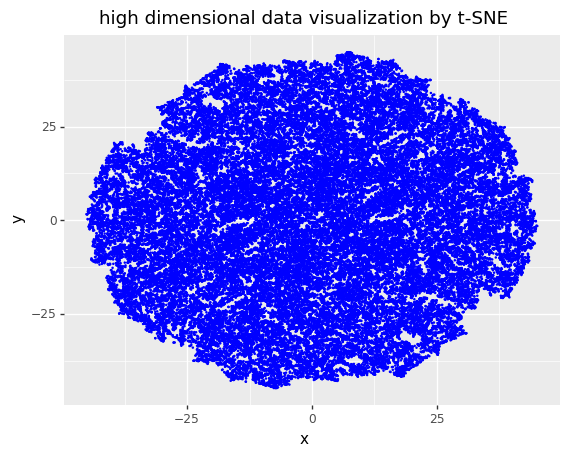
\includegraphics[scale=0.9]{tsne.png} 

\quad After deciding not doing outlier detection, we tried MLP with several different number of hidden layers and number of hidden neurons but they all converged to same testing accuracy very quickly. Then we tried logistic regression in R and found it showed around same testing accuracy as was in MLP model. We decided to use MLP in pre-game statistics for game result prediction since it is more versatile.

\quad The final weights for 10 features in 0-hidden-layer MLP are: \newpage

\textbf{Mean Weight vs Epoch\qquad \qquad Accuracy vs Epoch} \\
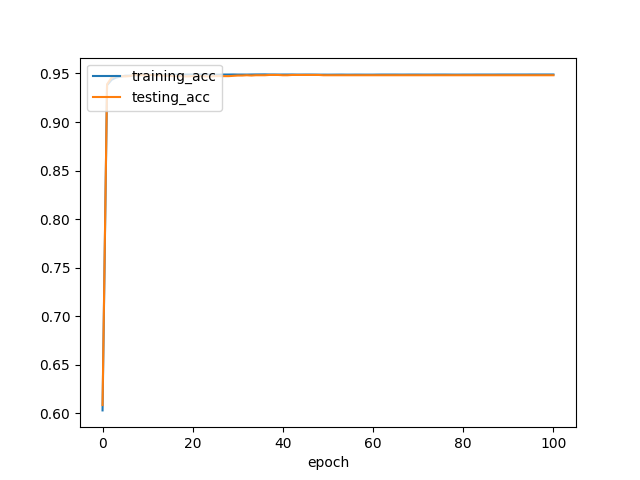
\includegraphics[scale=0.4]{postGame_0_1_compact_accuracy.png} 
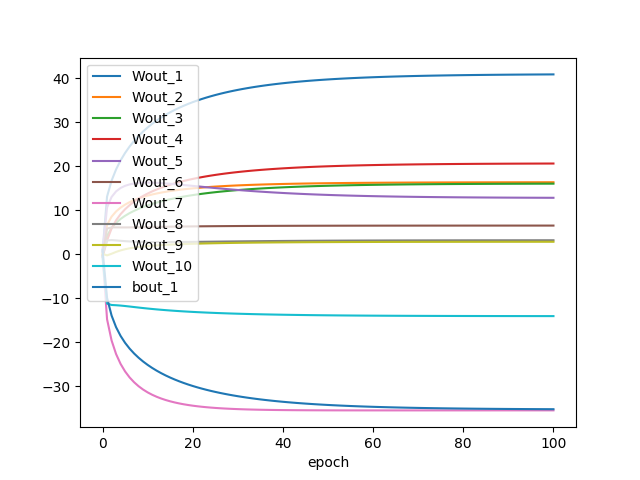
\includegraphics[scale=0.4]{postGame_0_1_detailed_weights.png} \\

\textbf{Individual Weights in Post-Game Stat MLP Game Prediction}


\begin{tabular}{llllllllll}
FG\%\_diff & 3P\%\_diff & FT\%\_diff  & OR\_diff   & DR\_diff \\
40.828392  & 16.331735  & 16.0064106  & 20.5814533 & 12.79597 
\end{tabular} 

\begin{tabular}{llllllllll}
AST\_diff &TO\_diff & STL\_diff & BLK\_diff& PF\_diff\\
6.48547268  &-35.493058 & 3.15093279 & 2.80670953 & -14.080395
\end{tabular}



\subsection{Results on pre-game statistics game results prediction}
\quad Combined versions of the MLP plots on pre-game data\footnote{Individual images can be found in \texttt{/mlp/NCAA\_preGame/plots/}.} for grid search on [1, 6] layer neuron and [1, 3] hidden layers are on the next two pages, where row number is the number of neurons per layer, and column number is the number of hidden layer. The plots for grid search on no hidden layer are on the page after. \newpage

\textbf{Mean Weights vs Epoch}

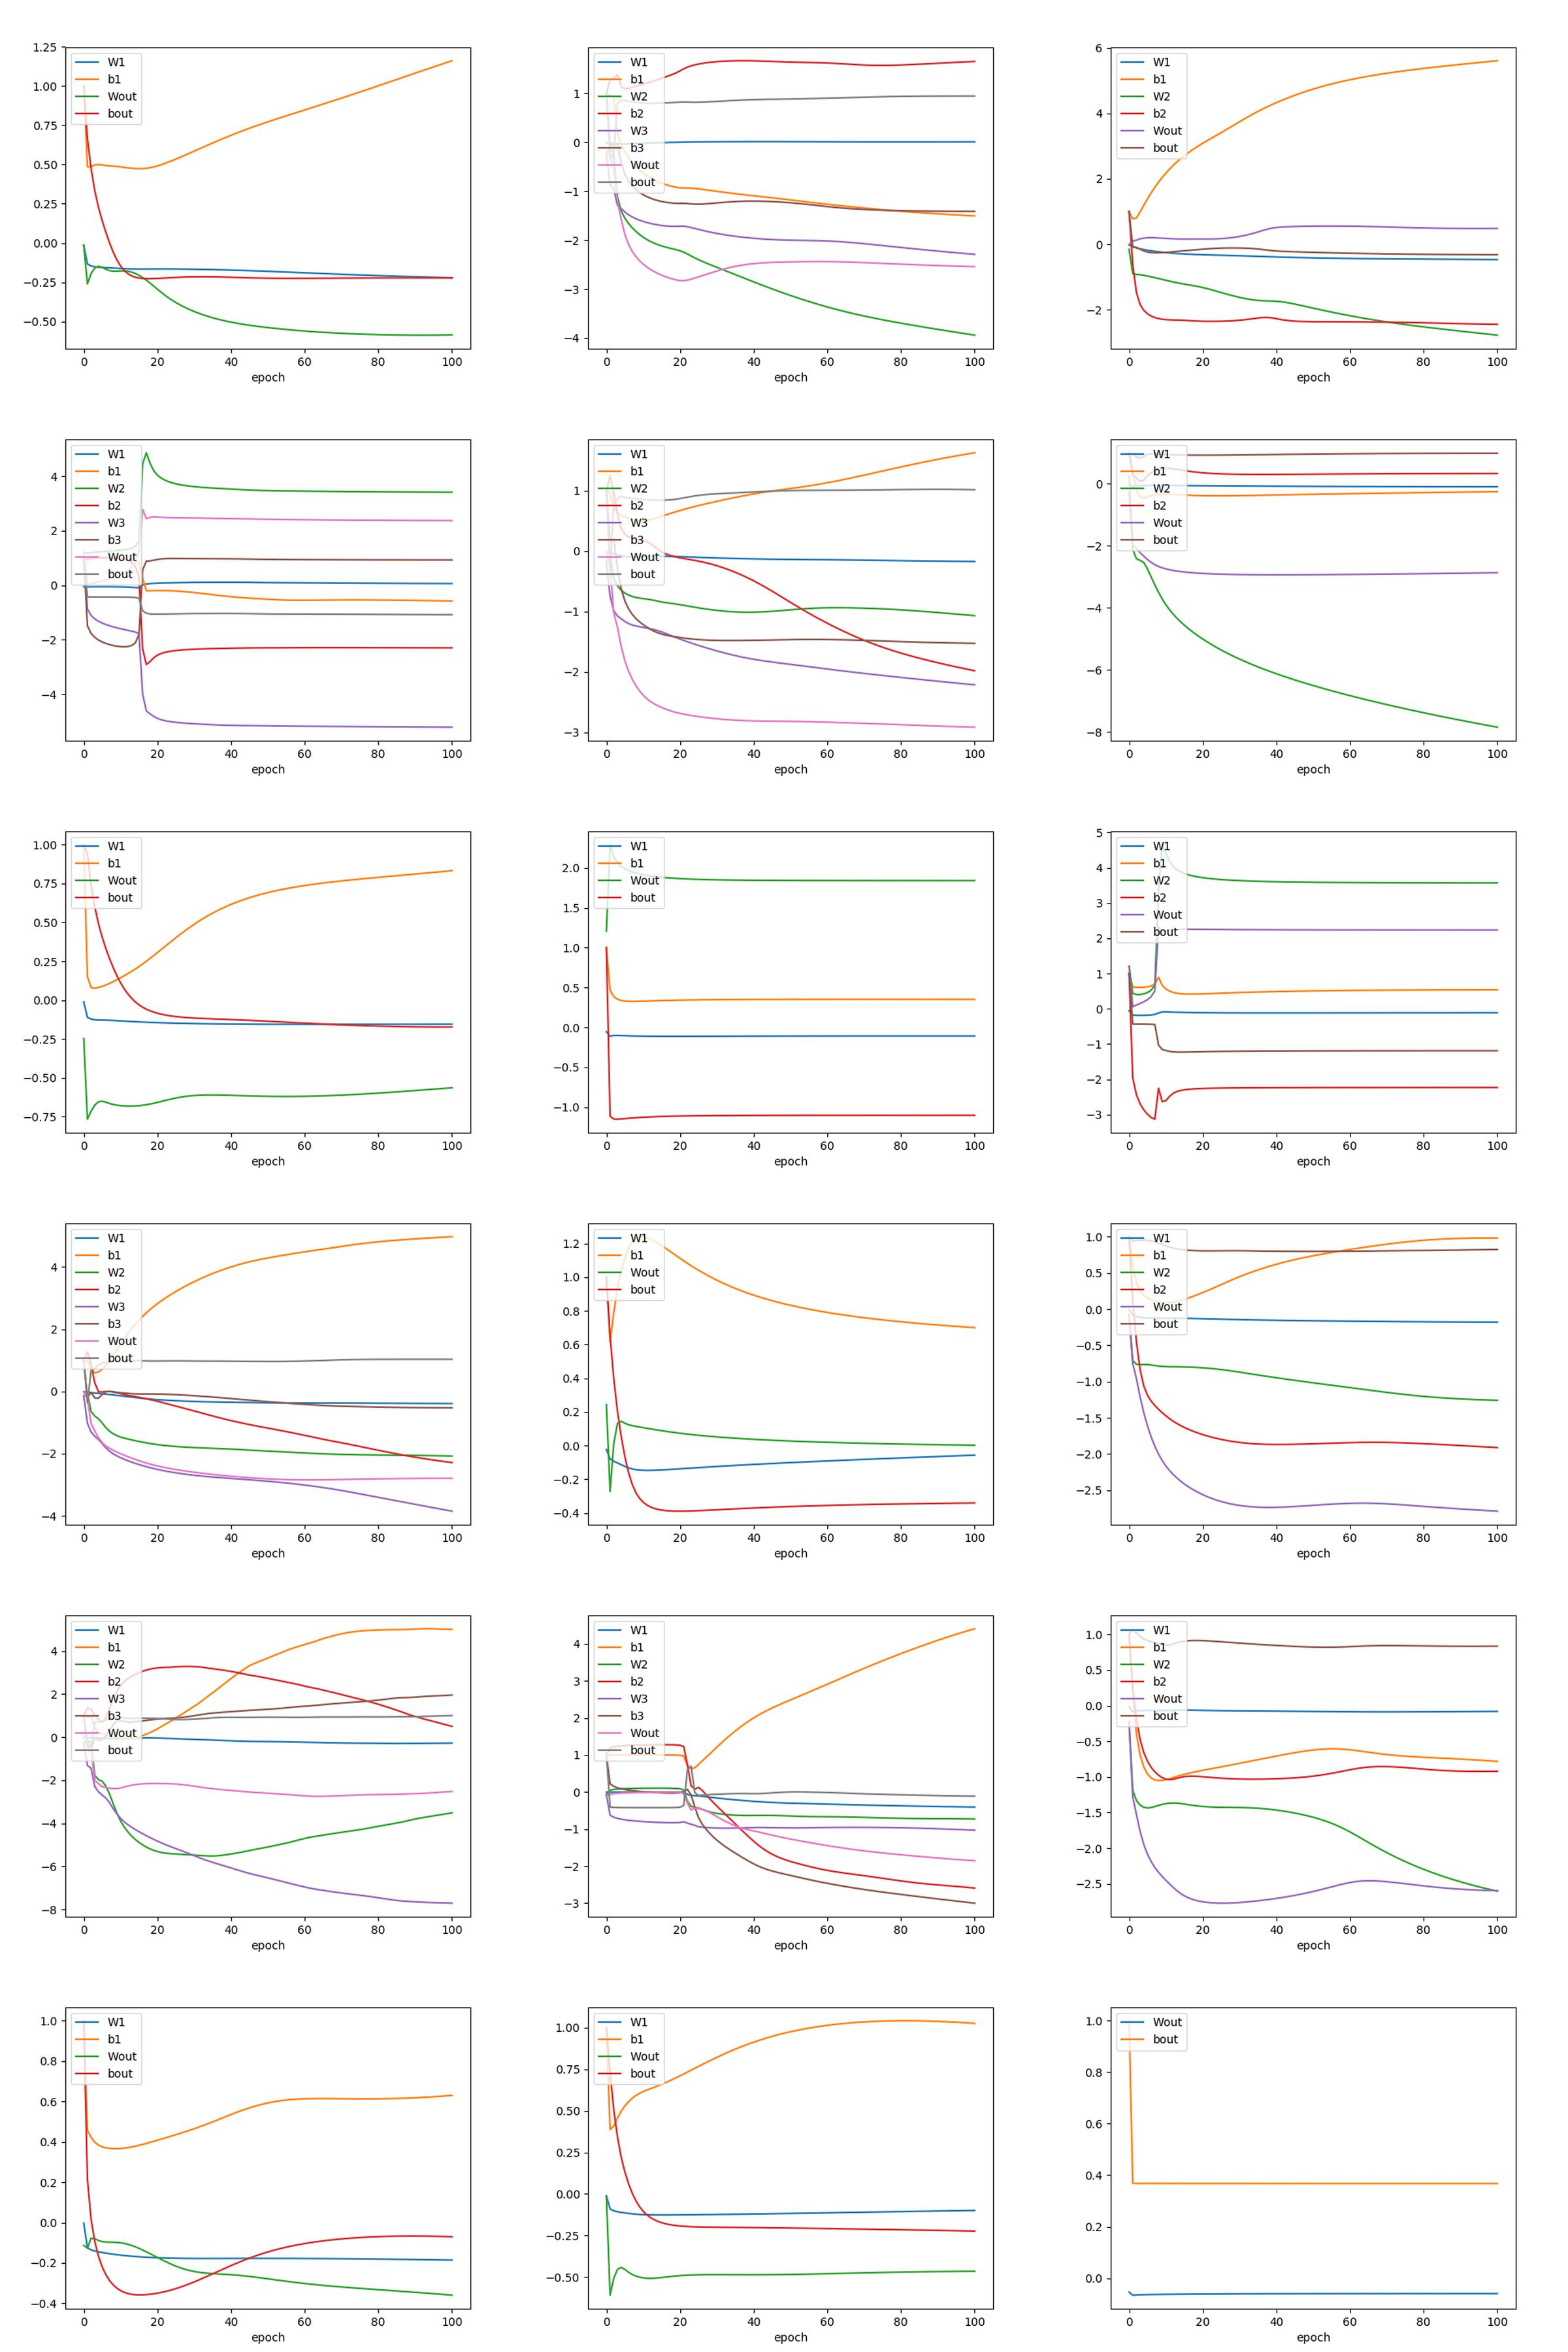
\includegraphics[scale=0.145]{NCAA_18_weights.jpg} \newpage 

\textbf{Accuracy vs Epoch}

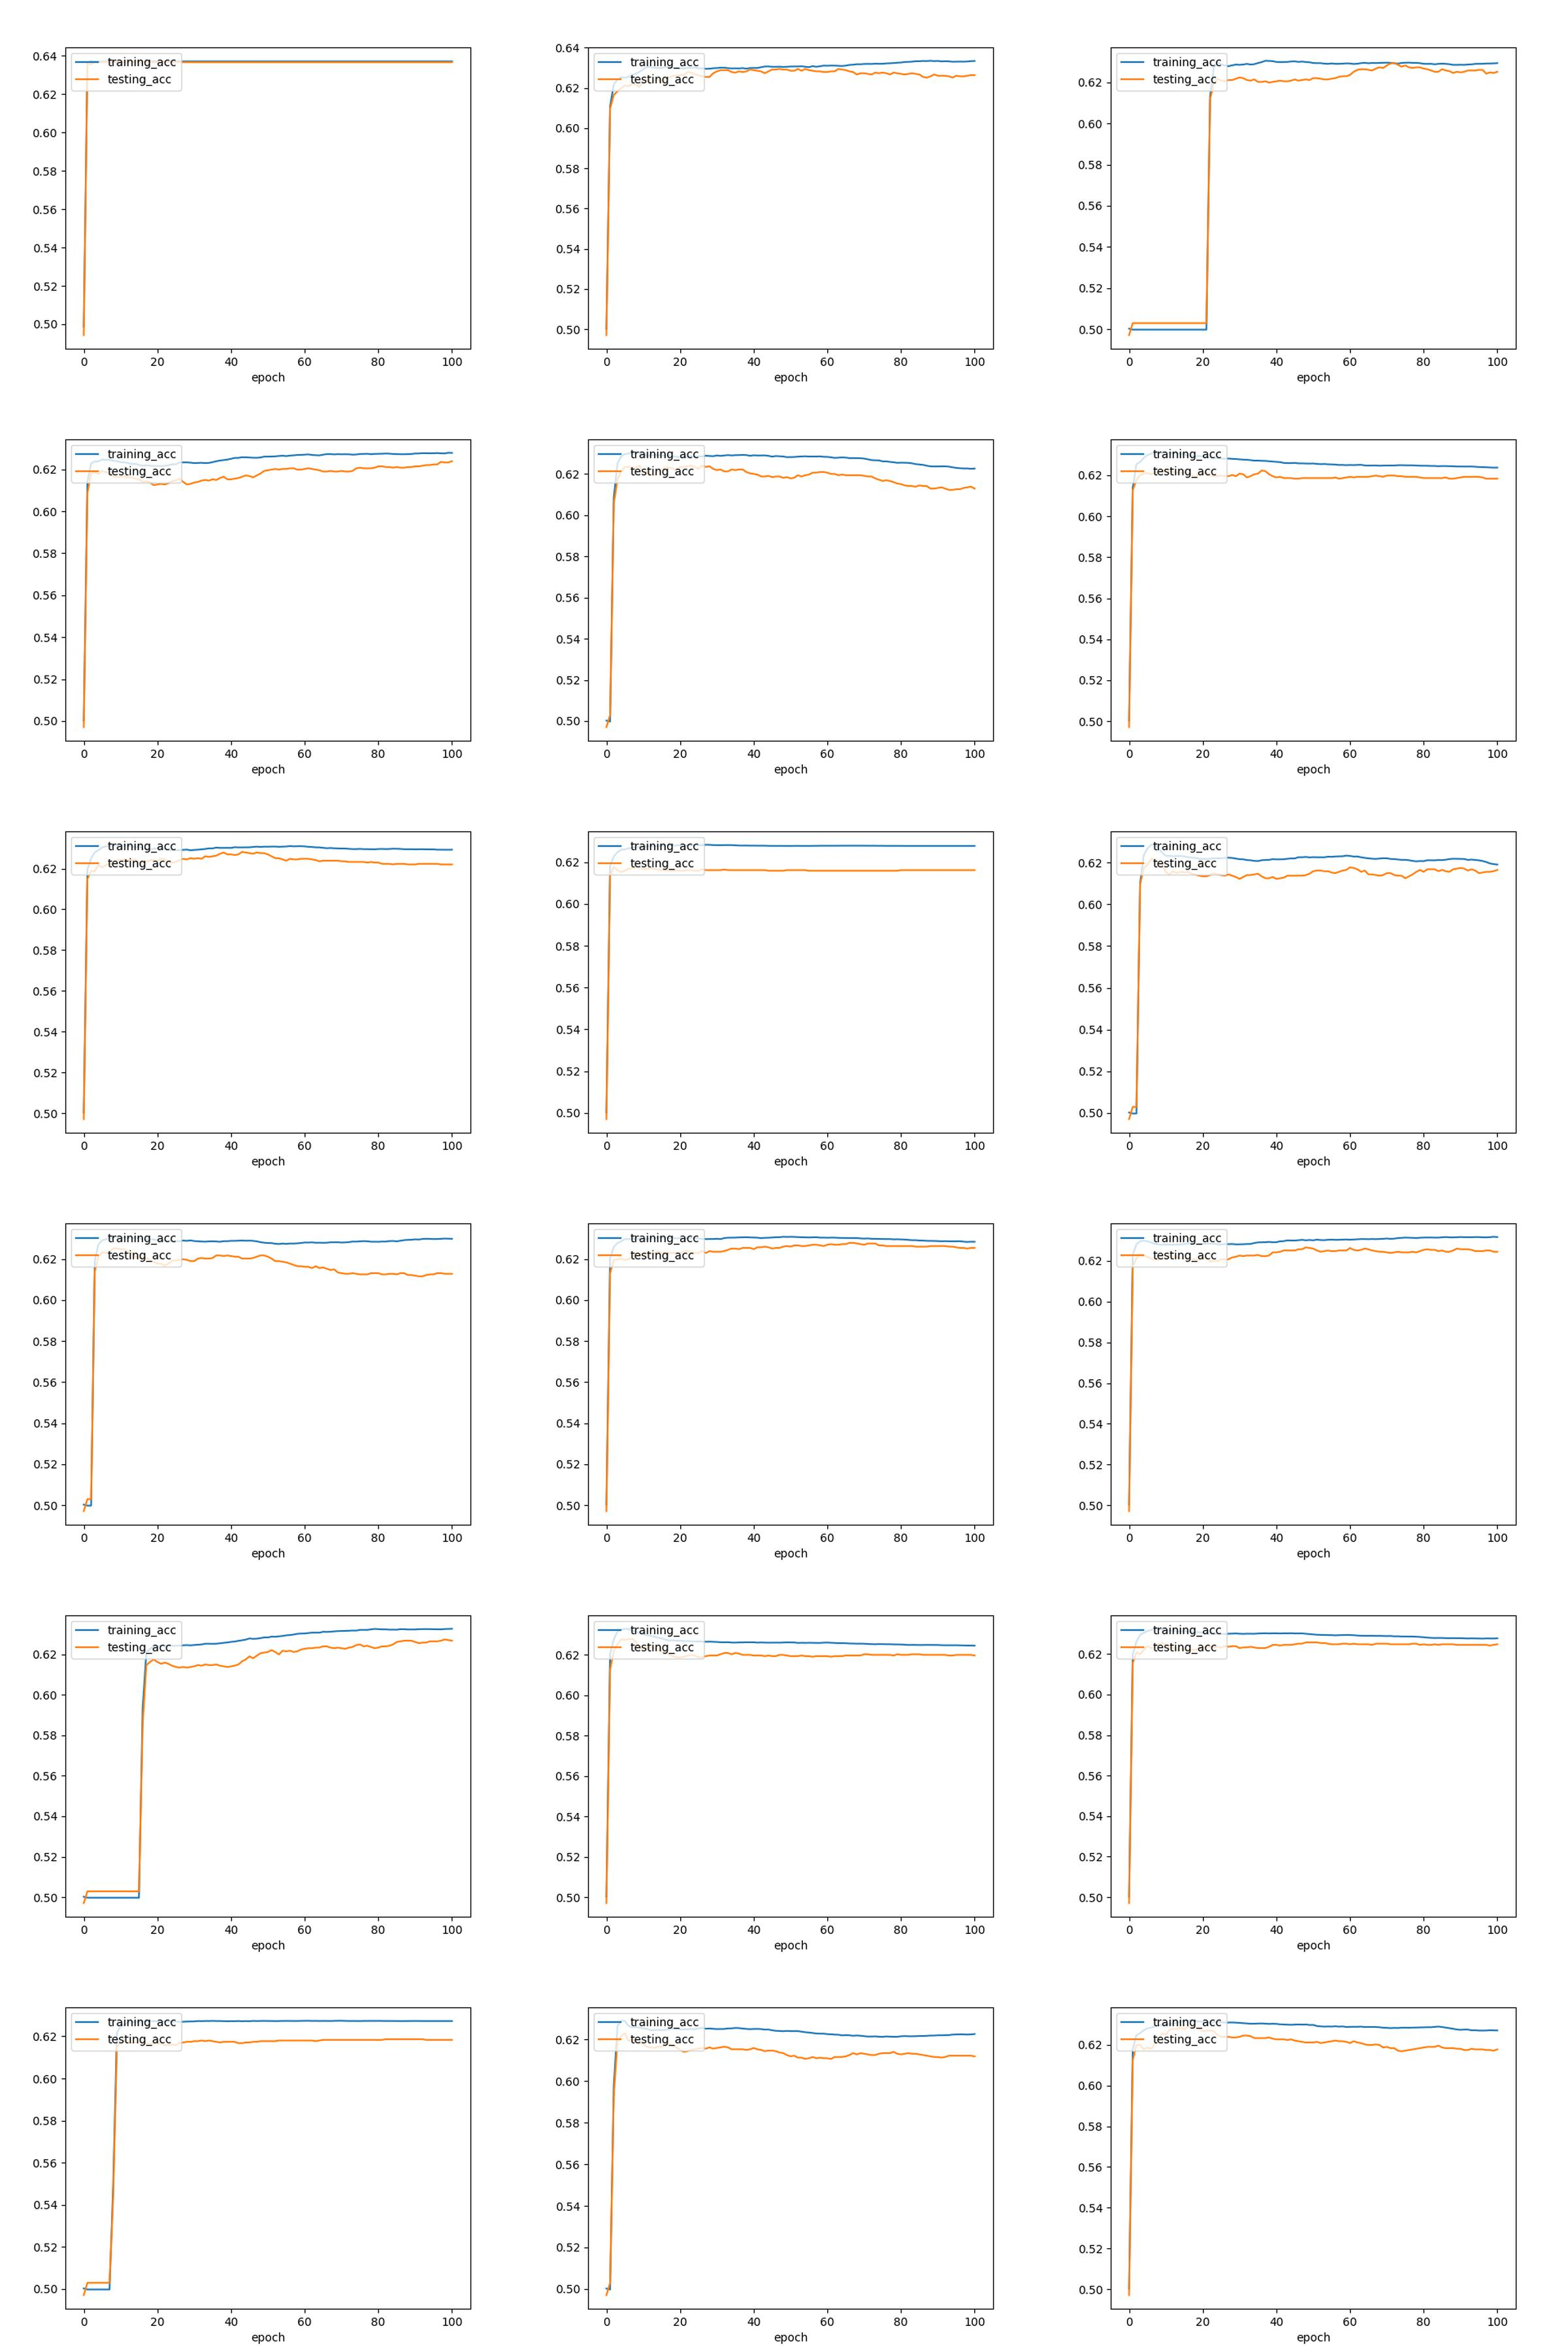
\includegraphics[scale=0.145]{NCAA_18_accuracy.jpg} \newpage

\textbf{Mean Weight vs Epoch\qquad \qquad Accuracy vs Epoch}

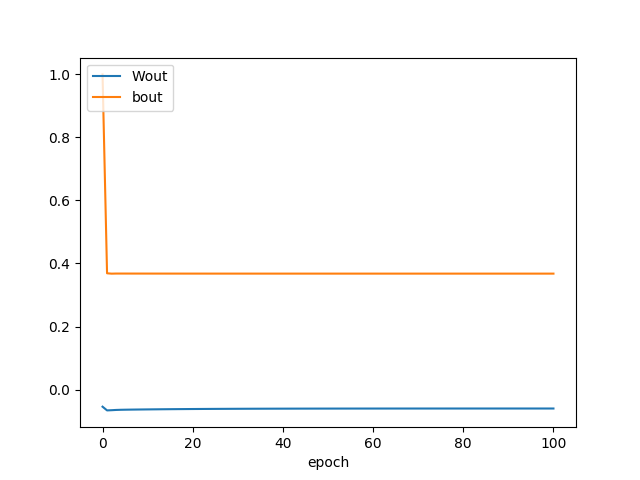
\includegraphics[scale=0.4]{NCAA_0_1_compact_weights.png} 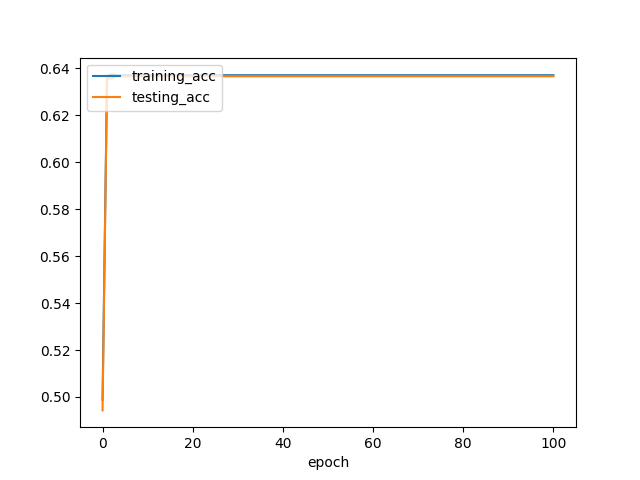
\includegraphics[scale=0.4]{NCAA_0_1_compact_accuracy.png} \\ 


\quad Results from running the logistic regression model are shown below:


\lstset{upquote=true}
\begin{lstlisting}[basicstyle=\small, numbers=left]
$ rscript logitReg/logitReg.R 
Running ./data_processing/output/post_game_team_diff.csv
Training Accuracy:	0.9488
Testing Accuracy:	0.9489
Running ./pre_game_teams.csv
Training Accuracy:	0.647
Testing Accuracy:	0.6032
\end{lstlisting}



\section{Discussion} 

\subsection{Conclusion}

\quad Since predicting game result is a problem of classification, we consider the logistic regression the optimal choice. But we initially decided to use ANN since logistic regression can be done through ANN with 0 hidden layer, and we want to test if using multiple hidden layers and multiple neurons has any effects on predicting accuracy.


\quad We noticed a huge drop from 95\% post-games testing accuracy in MLP to around 63\% pre-games testing accuracy. Such discrepancy can be explained in terms of uncertainty of NCAA’s games and our methods in generating expected team features. 

\quad The nature of NCAA complicated the prediction because NCAA has a higher rate of changing players in a team. We could only infer a new player’s post-game statistics by the average of the past instances of new players. But those data has a high variance, which means single player differs from one to one drastically. A replacing solution is to take the average of previous years, but such measure is the same as the what we took, and taking average from 2010 to 2017 would be closer to new players’ average post-game statistics. We haven’t found a better way to estimate pre-game new players’ statistics.

\quad A series of other problems arose as we proceeded our prediction. We weren’t satisfied with our testing accuracy at only 60\%. We found some similar studies on NBA game results prediction[10] and realized we didn’t do feature validation and feature selection before training. We have 21 features for each team (thus, 42 for 2 teams) in pre-game statistics prediction, but 3 of them belong to the same category and 1 of them (technical foul) should be intuitively insignificant to game result. Therefore, to double check the features we select can best explain the game result, we categorized 21 features into 10 groups, the features we used in post-game statistics game results prediction. We found an interesting phenomenon in post-game statistics game result prediction. Only 2 features have negative weights are TO\_diff and PF\_diff. It makes sense because turnovers and personal fouls has an negative impact on a team’s scoring. But we didn’t have sufficient time to do the further pre-game statistics game result after removing the insignificant features. \\

\subsection{Improvement}

\subsubsection{Data}

\quad Coach information is not used mainly because we failed to find out how to define a coach’s effect on a team. A team’s performance may have some relationship with the change of coach, but given the situation that NCAA team members change more frequently and each team are having an average of three new players that have never played before, it made it really hard to determine and implement the effect of a coach in mathematical form. One of the simple ways to represent this effect, for instance, would be using the winning rate of the coach’s team of last season, but we didn’t apply it in our model because if the coach was new to the league, then this feature would become not applicable. 


\quad In real world, the team playing at its home is often considered to have certain advantages and to be more likely to win if the rank of the team is close to, or even a little bit lower than its opponent [5]. In this case, the location of the game should play a somewhat important role in predicting the outcome of a game. We expect that adding location of the game into the feature matrix would somehow improve accuracy.


\quad The dataset provided by Kaggle contains a lot of information, from essential information such as player and game statistics to supplement information such as team names, cities and secondary games. After scanning through the whole dataset and considering our goal and time we had, we decided to only focus on features that directly relate to the performance of a team and could be expressed in math formulas.

\subsubsection{Goal}

\quad The current goal of the project is to predict the outcomes of the games that are listed in events files and accuracy is calculated through comparing our prediction with real results. An alternative way to set the goal consists of two parts: predicting all regular season games, and predicting tourney of which the teams that play are based on regular season results. This will make the project have more practical meanings. However, the rules and schedule of tourney were quite confusing, and unfortunately we didn’t notice it before we realize that we didn’t have much time left.

\subsubsection{Model}

\quad Since our model uses the features, the statistics of players, to predict an outcome of a game, our model would not take into account margin cases in which a team that is predicted to be weaker wins the stronger team and home-court advantage. To compromise these problems, we could have created a model using Markov Chain. [7]

\quad The goal is to find the transition matrices which represent the likelihood of team A being better than team B given that A beat B by x points . We can use a logistic model to obtain a smoother estimate of  the probabilities of  win rate. Then we can use these transition matrices with probabilities to predict the outcome of a game. To further make the predictions accurate for the matches in NCAA, we can deduce the transition matrices without home-advantage effect when we want to predict a game in a neutral-court game. [7]


\newpage

\section*{Author contributions}

Ming Cheng: Data Framing, Report

Xingwei Ji: Data preprocessing, outlier detection, Report

Xiaofang Jiang: Input refining, Report

Fangzhou Li: Project outline; Data preprocessing; Report

Diwen Lu: Data preprocessing; training

Paul Lu: Input refining, Report

Jiayi Xu: Data Framing, Report

Timothy Zhang: MLP \& Logistic Regression construction; training

Haibin Zhang: primary architecture, data set and filtrate

Feiwen Zheng: Input refining, Report \newpage



\section*{References (Samples)}
\qquad \qquad \qquad \qquad \qquad \qquad \qquad \qquad \qquad \qquad \qquad \qquad \qquad \qquad \qquad \qquad \qquad \qquad \qquad \qquad \qquad \qquad \qquad \qquad \qquad \qquad .
 
\small

[1]	NCAA Division I Men's Basketball Tournament (2018). Available: 

https://en.wikipedia.org/wiki/NCAA\_Division\_I\_Men\%27s\_Basketball\_Tournament. \\

[2]	Shi, Z., Moorthy \& S.,  Zimmermann, A. (2013) Predicting NCAAB match outcomes using ML techniques—some results and lessons learned. Proceedings of the MLSA Workshop at ECML/PKDD 2013

https://arxiv.org/pdf/1310.3607.pdf \\

[3]	Zimmermann, A. (2016) Basketball Predictions in the NCAAB and NBA: Similarities and Differences. Available: 

https://zimmermanna.users.greyc.fr/papers/journals/sadm2016.pdf.\\

[4]	Google Cloud \& NCAA® ML Competition 2018-Men's. Available: 

https://www.kaggle.com/c/mens-machine-learning-competition-2018/data. \\

[5]	Lopez, M.J. \& Matthews, G. (2014) Building an NCAA Men's Basketball Predictive Model and Quantifying Its Success. arXiv: 1412. 0248. Available:

            https://creativematter.skidmore.edu/cgi/viewcontent.cgi?article=1001\&context=math\_fac\_schol \\

[6]       Lo-Hua, Y. \& Anthony, L. (2015) A mixture-of-modelers approach to forecasting NCAA tournament outcomes. Available:

            https://www.lukebornn.com/papers/yuan\_jqas\_2014.pdf \\

[7]       S.P.Kvan and J.S.Sokol. (2016) A logistic regression/Markov Chain model for NCAA basketball. Naval Research Logistics, 53:788-803 Available:

            https://onlinelibrary.wiley.com/doi/epdf/10.1002/nav.20170 \\

[8]       Mark, B. \& Joel, S. (2010) An improved LRMC method for NCAA basketball predictions. Journal of Quantitative Analysis in Sports. Available:

https://www.degruyter.com/downloadpdf/j/jqas.2010.6.3/jqas.2010.6.3.1202/jqas.2010.6
.3.1202.pdf \\
	
[9]       Harish, S.B. \& Li-Hsuan, H. \& Sebastian R. (2015) Learning stochastic models for basketball substitutes from play-by-play data. In MLSA15, Workshop at ECML/PKDD.Available:

        	http://ceur-ws.org/Vol-1970/paper-08.pdf\\

[10]     Eric S.J. (2016) Predicting outcomes of NBA Basketball Games. Available:

https://library.ndsu.edu/ir/bitstream/handle/10365/28084/Predicting\%20Outcomes\%20of      \%20NBA\%20Basketball\%20Games.pdf?sequence=1\&isAllowed=y\\

\end{document}
